\chapter{\ifenglish Conclusions and Discussions\else บทสรุปและข้อเสนอแนะ\fi}

\section{\ifenglish Conclusions\else สรุปผล\fi}

จากผลการทดสอบกับผู้ใช้งานสรุปได้ดังนี้
เนื่องมาจากสถานการณ์โรคระบาดโควิด-19ทำให้การทดสอบระบบต้องทดสอบด้วยความล่าช้า
เนื่องจากไม่ได้ทำเรื่องเบิกเงินเพื่อสมัครสมาชิกนำแอพขึ้น play store ทำให้ต้องใช้การติดตั้งแบบ apk ไฟล์ผ่าน android studio
โดยต้องนัดเจอกันเพื่อติดตั้งแอพทดสอบ สถานการณ์โรคระบาดโควิด-19ทำให้การนัดเจอกันค่อนข้างยากขึ้นจึงได้รวมผู้เข้าร่วมทดสอบจำนวน 5 คน เป็นระยะเวลาทดลอง20นาที หลังจากนั้นให้ผู้ใช้ตอบแบบสอบถาม
ความพึงพอใจหลังใช้งานโดยรายละเอียดแบบสอบถามแสดงไว้ในภาคผนวก ก. และได้ผลดังนี้ ดังรูปที่
5.1


\begin{figure}
    \begin{center}
      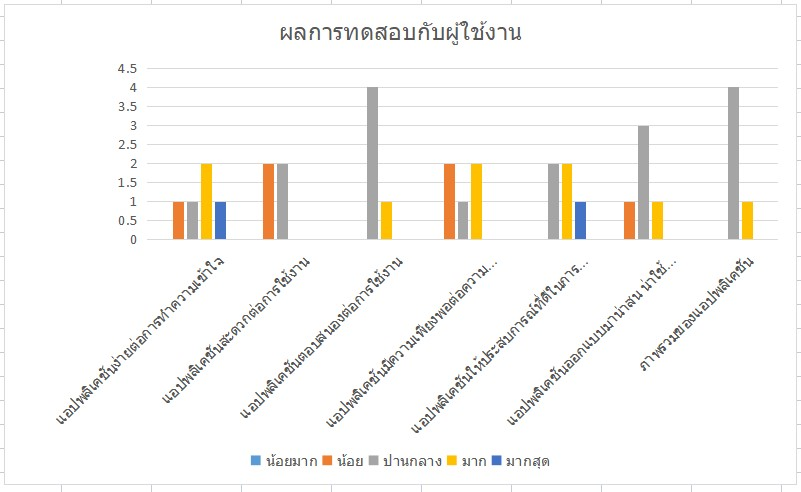
\includegraphics[width=1\textwidth]{./image/form/result_reviews.jpg}
    \end{center}
    \caption[ผลการทดสอบกับผู้ใช้งาน]{ผลการทดสอบกับผู้ใช้งาน}
    \end{figure}

    จากกราฟผลการทดสอบกับผู้ใช้งานสามารถแสดงให้เห็นคร่าวๆว่าแอปพลิเคชันสามารถทำงานต่างๆได้ดีโดยรวม 
    ผู้ใช้สามารถทำความเข้าใจได้ไม่ยาก ความเร็วในการตอบสนองการโหลดเนื้อหาได้เร็วปานกลาง การออกแบบหน้าตาของแอปพลิเคชันพอใช้ได้
    สามารถให้ประสบการณืใช้งานกับผู้ใช้ค่อนข้างดี 

    จากการพัฒนาโครงงาน Wongwien ระบบที่ได้สามารถทำงานตามวัตถุประสงค์ของโครงงานได้นั่นคือได้แพลตฟอร์มที่สามารถใช้ใน
    การรีวิวเรื่องต่างๆต่างหมวดหมู่ สามารถตั้งกระทู้เพื่อไขข้อสงสัยต่างๆ สามารถค้นหารีวิว สามารถสนทนาขอรับคำปรึกษาและ
    สามารถเพิ่มวิธีการเข้าใช้งานระบบผ่านแฟตฟอร์มอื่นเพื่อความสะดวกสบาย ระบบสามารถทำงานแบบออฟไลน์ได้ถ้าหากเคยมีการใช้งานมาก่อนจะเก็บเนื้อหาล่าสุดไว้

\section{\ifenglish Challenges\else ปัญหาที่พบและแนวทางการแก้ไข\fi}

ในการทำโครงงานนี้ พบว่าเกิดปัญหาหลักๆ ดังนี้
\begin{enumerate}
    \item ปัญหาด้านการทดสอบระบบ อันเนื่องมาจากสถานการณ์โรคระบาดโควิด-19ทำให้การทดสอบระบบต้องทดสอบด้วยความล่าช้า
    เนื่องจากไม่ได้ทำเรื่องเบิกเงินเพื่อสมัครสมาชิกนำแอพขึ้น play store ทำให้ต้องใช้การติดตั้งแบบ apk ไฟล์ผ่าน android studio
    โดยต้องนัดเจอกันเพื่อติดตั้งแอพทดสอบ สถานการณ์โรคระบาดโควิด-19ทำให้การนัดเจอกันค่อนข้างยากขึ้น
    \item การทำงานของแอพพลิเคชันเมื่อมีอินเตอร์เน็ตที่ช้าทำให้การดึงข้อมูลช้าตามอาจสร้างความลำคาญกับผู้ใช้ได้
    \item ในการทำโปรเจคในครั้งนี้เรื่องของการแชร์ไปยังแอปพลิเคชันอื่นรอรับการแชร์ที่สมบูรณ์เมื่อเเชร์ผ่านอีเมล
\end{enumerate}
\section{\ifenglish%
Suggestions and further improvements
\else%
ข้อเสนอแนะและแนวทางการพัฒนาต่อ
\fi
}

ข้อเสนอแนะเพื่อพัฒนาโครงงานนี้ต่อไป มีดังนี้
\begin{enumerate}
    \item ควรทำการพัฒนา UI ให้สวยงามน่าใช้งานมากกว่านี้และควรมีฟังชันอื่นๆที่น่าสนใจเพื่อดึงดูดผู้ใช้งาน
    \item ควรเพิ่มความสามารถในการปรับแต่งการรีวิวให้มันมีมากกว่านี้
\end{enumerate}
